% !TEX encoding = UTF-8 Unicode
\documentclass[
10pt,
aspectratio=169,
]{beamer}
\setbeamercovered{transparent=10}
\usetheme[
%  showheader,
%  red,
  purple,
%  gray,
%  graytitle,
  colorblocks,
%  noframetitlerule,
]{Verona}

\usepackage[T1]{fontenc}
\usepackage[utf8]{inputenc}
\usepackage{lipsum}
%%%%%%%%%%%%%%%%%%%%%%%%%%%%%%%
% Mac上使用如下命令声明隶书字体,windows也有相关方式,大家可自行修改
%\providecommand{\lishu}{\CJKfamily{zhli}}
%%%%%%%%%%%%%%%%%%%%%%%%%%%%%%%
\usepackage{tikz}
\usetikzlibrary{fadings}
%
%\setbeamertemplate{sections/subsections in toc}[ball]
%\usepackage{xeCJK}
%\usepackage[shortlabels]{enumitem} 
\usepackage{adjustbox} % Shrink stuff
\usepackage{listings}
\usepackage{caption}
\usepackage{subcaption}
\usefonttheme{professionalfonts}
\def\mathfamilydefault{\rmdefault}
\usepackage{amsmath}
\usepackage{multirow}
\usepackage{booktabs}
\usepackage{bm}
\setbeamertemplate{section in toc}{\hspace*{1em}\inserttocsectionnumber.~\inserttocsection\par}
\setbeamertemplate{subsection in toc}{\hspace*{2em}\inserttocsectionnumber.\inserttocsubsectionnumber.~\inserttocsubsection\par}
\setbeamerfont{subsection in toc}{size=\small}
\AtBeginSection[]{%
	\begin{frame}%
		\frametitle{Outline}%
		\textbf{\tableofcontents[currentsection]} %
	\end{frame}%
}

\AtBeginSubsection[]{%
	\begin{frame}%
		\frametitle{Outline}%
		\textbf{\tableofcontents[currentsection, currentsubsection]} %
	\end{frame}%
}

\title{Manejo de el tiempo para investigadores}
\subtitle{Herramientas para la elaboraci\'on de la propuesta}
\author[L.M.]{Luis Alejandro Morales, Ph.D.}
\mail{lmoralesm@unal.edu.co}
\institute[UNAL]{Facultad de Ingenier\'ia, Departamento de Ingnenier\'ia Civil y Agr\'icola\\
Universidad Nacional de Colombia, Bogot\'a}
\date{\today}
\titlegraphic[width=3cm]{logo_01u}{}

%%%%%%%%%%%%%%%%%%%%%%%%%%%%%%%%
% ----------- 标题页 ------------
%%%%%%%%%%%%%%%%%%%%%%%%%%%%%%%%
% New commands
\newcommand{\gi}{\texttt{Git}}
\newcommand{\gih}{\texttt{GitHub}}
\newcommand{\co}[1]{\alert{\textbf{\large \texttt{#1}}}}
\begin{document}



\maketitle

%%% define code
\defverbatim[colored]\lstI{
	\begin{lstlisting}[language=C++,basicstyle=\ttfamily,keywordstyle=\color{red}]
	int main() {
	// Define variables at the beginning
	// of the block, as in C:
	CStash intStash, stringStash;
	int i;
	char* cp;
	ifstream in;
	string line;
	[...]
	\end{lstlisting}
}
%%%%%%%%%%%%%%%%%%%%%%%%%%%%%%%%
% ----------- FRAME ------------
%%%%%%%%%%%%%%%%%%%%%%%%%%%%%%%%

%---
\section{Generalidades}

\begin{frame}[c]{La rueda de la vida}
De 0 a 10 califique que tan importante es cada secci\'on de la rueda.
\begin{center}
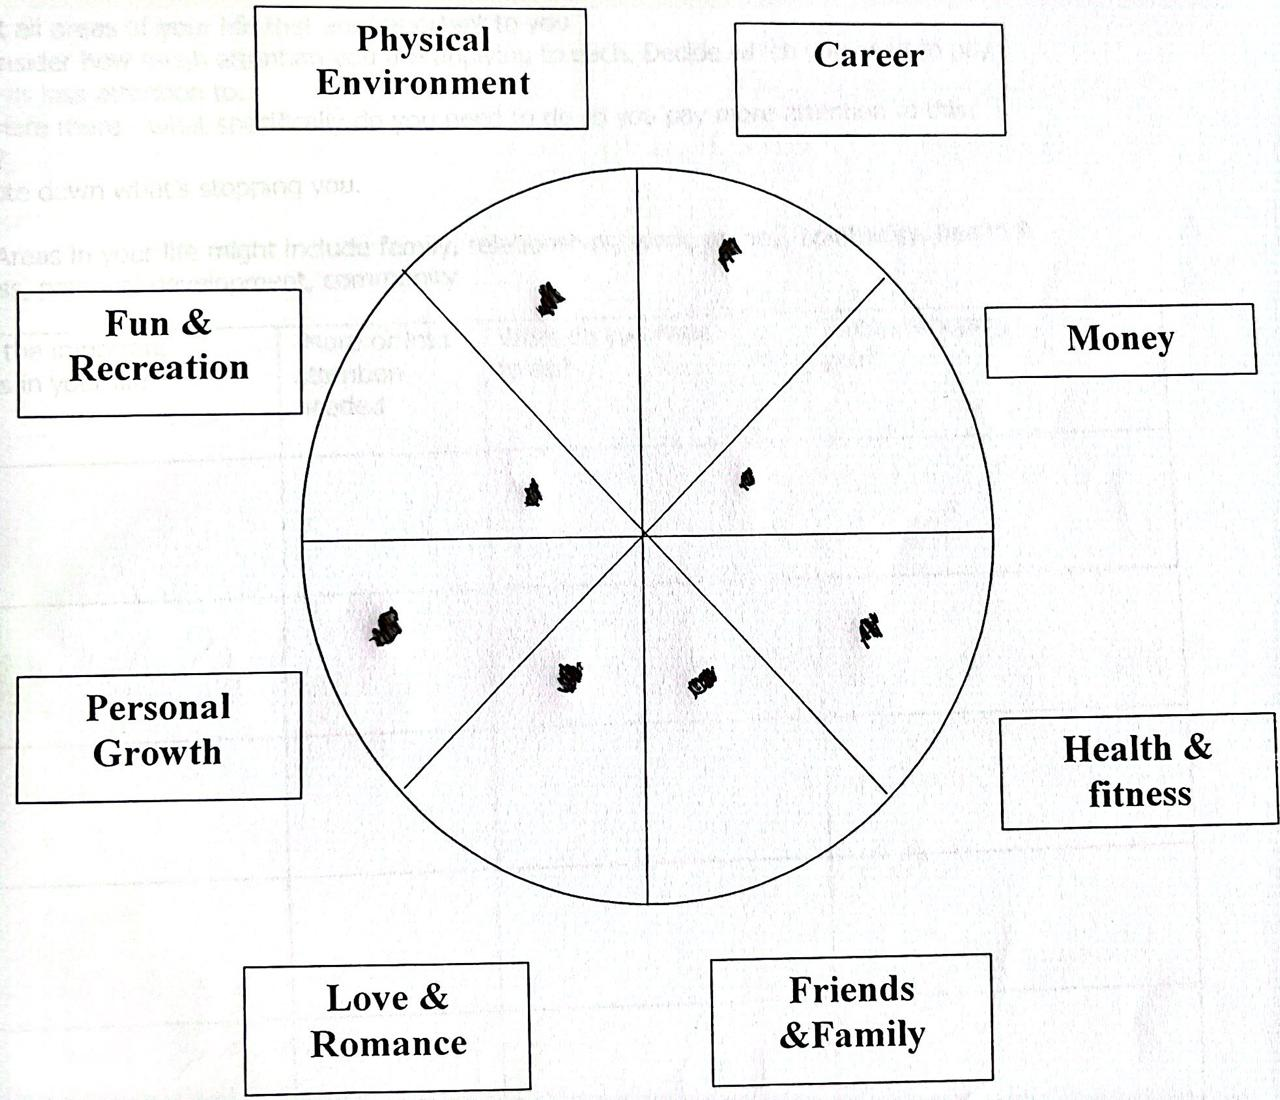
\includegraphics[width=0.5\textwidth]{wheel.jpeg}
\end{center}
\vspace{-0.2cm}
\alert{Se debe procurar que la rueda sea lo mas uniforme posible.}
\end{frame}

\begin{frame}[c]{Productividad}
\huge{
\begin{equation*}
\text{Productividad}\ \propto\  \text{tiempo x eficiencia}
\end{equation*}}
\large
La eficiencia, depende de:
\begin{itemize}
\item Priorizaci\'on
\item Planeaci\'on y organizaci\'o
\item Intensidad en la concentraci\'on
\item Involucramiento de otros
\item No perder el norte
\item Buen manejo del tiempo.
\end{itemize}
\huge{
\begin{equation*}
\text{Manejo del tiempo}\ = \text{Planeaci\'on y organizaci\'on}
\end{equation*}}

\end{frame}


\begin{frame}[c]{Workflow}
\centering
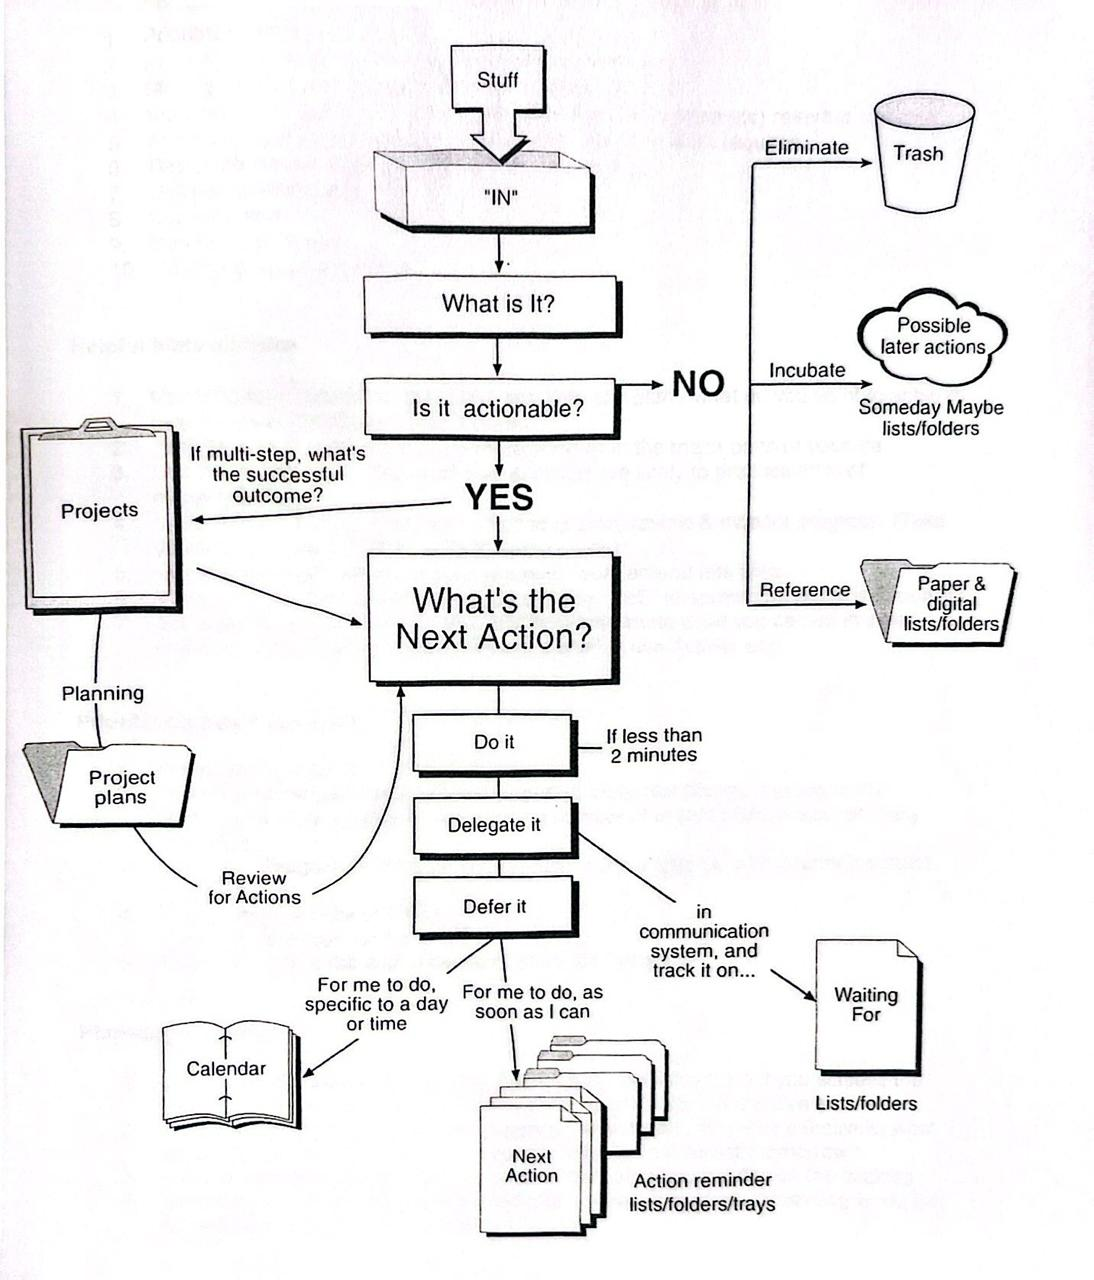
\includegraphics[width=0.45\textwidth]{workf.jpeg}
\end{frame}
%---
\section{Estrategias para planear sus actividades}
\begin{frame}[c]{Defina us objetivos}
La planeaci\'on inicia con un objetivo. Existen diferentes objetivos:
\begin{enumerate}
\item \alert{Objetivos a largo plazo}: Son una combinacion de objetivos tangibles (e.g. ser promocionado en su trabajo) e intangibles (e.g. ser feliz). Estos pueden cambiar con el tiempo y se deben revisar periodicamente. Al definir estos objetivos, usted se esta definiendo que quiere ser en 3 o 5 a\~nos.
\item \alert{Objetivos a mediano plazo}: Son tareas a realizar en seis meses o un a\~no. Generalmente se alcanzan al lograr una serie de objetivos de corto plazo. E.g. escribir un articulo, realizar los experimentos de mi tesis. 
\item \alert{Objetivos de corto plazo}: Estos objetivos se logran en un mes o una semana. Son establecidos como pasos para alcanzar objetivos de mediano plazo. E.g. hacer las figuras del articulo, escribir la introducci\'on del articulo. 
\end{enumerate}
\end{frame}

\begin{frame}[c]{El poder del tres}
Defina lo siguiente:
\begin{enumerate}
\item El top 3 de las prioridades para este a\~no o el proximo a\~no.
\item El top 3 de las prioridades para los pr\'oximos tres meses. 
\item El top 3 de las prioridades para el pr\'oximo mes.
\item El top 3 de las prioridades para la pr\'oxima semana.
\item El top 3 de las prioridades para hoy.
\end{enumerate}
\end{frame}


\begin{frame}[c]{Diez aspectos del manejo de tiempo}
\begin{enumerate}
\item Priorize su trabajo.
\item Conozca la cantidad de tiempo que las actividades requieren para realizarce.
\item Haga programas reales de tiempo (e.g. dia, semana, proyecto)
\item Haga que sus reuniones sean breves y relevantes.
\item Determine que recursos requiere una tarea para realizarla.
\item Disene estrategias simples para anotar informacion basica.
\item Delegue efectivamente.
\item Concentrese.
\item Maneje su agenda de apuntes.
\item Controle sus pequenos malos habitos. 
\end{enumerate}
\end{frame}

\begin{frame}[c]{Escoger que hacer}
\begin{itemize}
\item \alert{Decir no}: Es importante aprender a decir que no. No es posible hacer todo y estar disponible para todos. Esto permite enfocarse en lo que es importante. Para esto necesario establecer prioridades.
\item \alert{Maximizar beneficios}: Dada las restricciones de tiempo, es imposible hacer todo perfecto. Decida que debe ser llevado a la perfecci\'on y que no. 
\item \alert{Desconectese}: En un mundo hiperconectado, es necesario desconectarse para evitar interrupciones y aumentar la productividad.
\end{itemize}
\end{frame}


\begin{frame}[c]{Tips importantes}
\begin{enumerate}
\item Establesca un plan a largo plazo para tener claridad de sobre sus objetivos. ¿Que quiere obtener en los proximos 6 meses? Escriba esto.
\item Confirme cuales son sus principales objetivos en su vida.
\item Use la regla 20/80: El 20\% de todas sus actividades posiblemente produciran el 80\% de resultados significativos en su vida. 
\item Revise su plan frecuentemente y monitoree el avance. Para esto, vaya a un cafe, a una caminata, etc.
\item Determine cual su preferencia: madrugar o trasnochar. La que garantice un mejor trabajo.
\item Cuanto dice NO a algo, puede decir SI a algo que es importante.
\item Establezca tiempos reales de trabajo para una actividad.  Se tiende a sobreestimar el tiempo que requiere una actividad.  
\end{enumerate}
\end{frame}

\begin{frame}[c]{Ejercicio}
Escriba su top 3 de sus objetivos:
\begin{itemize}
\item A largo plazo
\item A mediado plazo
\item A corto plazo.
\end{itemize}
\end{frame}


%---
\section{Manejar el tiempo diario}
\begin{frame}[c]{Encontrar tiempo disponible}
Para trabajar de una manera eficiente y creativa, es necesario bloques de tiempo sin interrupciones. Esto se logra:
\begin{itemize}
\item \alert{Controlando el e-mail}: Establezca horas especificas del dia para revisar su e-mail. 
\item \alert{Llegue temprano a su oficina}: Evita el ruido que producen otras personas en su zona de trabajo.
\item \alert{Pongale seguro a la puerta}: Esto evita interrupciones de su preciado tiempo. 
\item \alert{Establezca tiempos en los que es inacesible}: Controla de manera efectiva el trabajo profundo. 
\end{itemize}
\end{frame}

\begin{frame}[c]{Rote sus tareas}
\begin{itemize}
\item Si usted se encuentra aburrido haciendo una unica tarea por un tiempo largo, asegurese de tener otras tareas por hacer.
\item Multitarea no es recomendable cuando se hace mas de una tarea a la vez (por periodos cortos de tiempo).
\item Es recomendable tener 3 o 4 tareas en las cuales es posible trabajar (una a la vez) por periodos largos de tiempo (e.g. 2 horas).
\end{itemize}
\end{frame}

\begin{frame}[c]{Establezca prioridades}
\begin{itemize}
\item Con base en sus objetivos, establesca que debe hacer y cuando. Siga el clasico \alert{KISS} (Keepe It Simple, Stu**). 
\item Establezca el siguiente cuadro y clasifique sus tareas de acuerdo con este.
\begin{center}
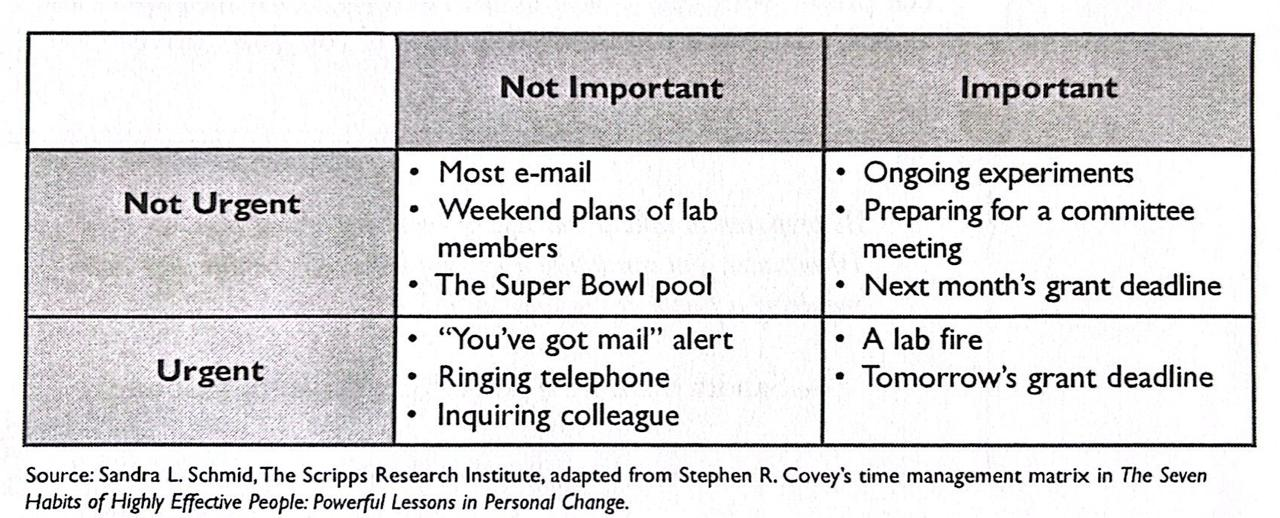
\includegraphics[width=0.6\textwidth]{imUr.jpeg}
\end{center}
\item Controle lo que esta en el cuadrante no urgente/no importante.
\item \alert{Para una maxima eficiencia, la mayor parte del tiempo se debe invertir en el cuadrante: no urgente/importante.}
\end{itemize}
\end{frame}

\begin{frame}[c]{Establezca prioridades}
Para aquellas tareas importante pero no urgentes, recuerde:
\begin{itemize}
\item Planear con anticipaci\'on y conocer los plazos de terminaci\'on.
\item Establecer periodos de tiempo para tareas especificas.
\item Divida tareas grandes en tareas peque\~nas (divide y conquistaras).
\item Delegue tareas.
\item Complete las tareas a tiempo. 
\end{itemize}
\end{frame}


\begin{frame}[c]{Seis elementos para priorizar el trabajo}
\begin{enumerate}
\item Tenga presente la idea general.
\item Entienda las diferencias entre urgente e importante. Cosas que son muy importantes, rara vez son urgentes.
\item Desarrolle la capacidad para enfocarse en una tarea (importante).
\item Enfoquese en el poder de 3.
\item Planee sus actividades de la semana.
\item Cada manana o al final del dia anterior, planee su dia.  
\end{enumerate}
\end{frame}

\begin{frame}[c]{To do list}
Defina lo siguiente:
\begin{itemize}
\item Haga su lista con papel y lapiz, no en el computador.
\item No reescriba su lista todos los dias.
\item Sea selectivo en lo que va en la lista.
\item Tenga otro lugar para escribir nuevas ideas.
\item Mantenga sus tareas cortas y especificas.
\item Recorra la lista en el orden en que esta; luego escoja.
\item Siempre inicie desde el principio.
\item Use esta misma tecnica para su e-mail y su bandeja de entrada. 
\end{itemize}
\end{frame}

\begin{frame}[c]{¿Como planear su dia?}
\begin{enumerate}
\item Liste todas las tareas/actividades que tiene que realizar hoy. Marque el top 5 y trabaje en cada una de ellas sequencialmente. 
\item Al final del dia revise su progreso. ¿Que ayudo en la realizacion de las actividades? ¿Que haria diferente?
\item Aparte momento del dia para trabajar durante una hora en tareas acumuladas
\item Tome un descanso de las tareas mas demandantes, esto agilizara el trabajo. 
\end{enumerate}
\end{frame}


\begin{frame}[c]{Aproveche al maximo el tiempo disponible}
Es importante encontrar maneras de hacer uso del tiempo de una manera \alert{eficiente} y \alert{productiva}.
\begin{itemize}
\item \alert{Eficiencia}: La gente exitosa tiende a ser eficiente. Crean bloques de tiempo de trabajo profundo sin interrupciones.
\begin{itemize}
\item Cree un ambiente propicio para la productividad. Evite el desorden y el ruido. Busque el lugar o el tiempo adecuado.
\item Proteja su tiempo mas preciado para trabajar en tareas criticas (e.g. escritura, programci\'on)
\item No permita interrupcion durante sus horas protegidas; concentrese. 
\item Establezca limites de tiempo o el tiempo requerido para completar una tarea.
\item Eliminar tareas que no sean necesarias.
\item Evite la dilacion de las tareas. Inicie las tareas con anticipacion; aquella que tienen un plazo.
\item Estructure y supervise reuniones.
\item Delegue trabajo.
\item Haga una llamada en lugar de conversar por e-mail.
\item Obtenga una conexion de Internet de alta velocidad. 
\end{itemize}
\item La gente exitosa adem\'as utiliza cualquier espacio de tiempo libre para trabajar. En 10 o 15 minutes, mientras esta esperando para una cita por ejemplo, es posible, escribir un email, hacer una llamada, llenar una forma, etc
\end{itemize}
\end{frame}

\begin{frame}[c]{Ejercicio}
Haga un listado de todas sus tareas a realizar en los  pr\'oximos 30 dias y clasifiquelas de acuerdo con la tabla mostrada
\end{frame}

\begin{frame}[c]{Ejercicio}
Hacer lo siguiente:
\begin{enumerate}
\item Escriba las actividades  que tiene que hacer hoy y el intervalo de tiempo.
\item Escriba las actividades a realizar esta semana y los dias en que se realizaran.
\item Escriba las actividades a realizar este mes.
\item Escriba las actividades a realizar en los pr\'oximos 6 meses y los meses en que las terminar\'a. 
\end{enumerate}
\end{frame}

%----
\section{Manejo de tiempo en ambientes espec\'ificos}
\begin{frame}[c]{Academia en investigaci\'on}
\begin{itemize}
\item Establezca tiempo limites para tareas que no sean academicas.
\item Cuando el tiempo se termina para una una determinada tarea, siga con la proxima tarea en su programacion diaria. 
\item Lo anterior sirver para iniciar cada dia con una serie de tareas nuevas y no las del dia anterior.
\end{itemize}
\end{frame}

\begin{frame}[c]{Hogar y oficina}
\begin{itemize}
\item \alert{Comunicacion familiar}

\begin{itemize}
\item Comparta sus objetivos a mediano y largo plazo con su familia.
\item Ponga un calendario en su casa con sus plazos de entrega claves. 
\item Programe actividades con su familia y cumplalas.
\item Si tiene un viaje de trabajo, conviertalo en unas pequenas vacaciones para usted y su pareja.
\item Involucre a su pareja en su trabajo. E.j. pidale el favor que lea sus escritos. 
\end{itemize}
\end{itemize}
\end{frame}

\begin{frame}[c]{Hogar y oficina}
\begin{itemize}
\item \alert{Balance entre el trabajo y sus hijos}
\begin{itemize}
\item La crianza puede complicar el trabajo. Sin embargo los ninos traen alegria y motivacion para ser m\'as eficientes.
\item Cuando su presupuesto lo permita, contre una ninera o una persona que le ayude con las labores del hogar. 
\item Salga a comer con su familia una vez a la semana; estos son actividades que todos disfrutan.
\item A veces es conveniente comer comida para llevar a la casa. Este tiempo se puede invertir en hablar con su pareja o en tiempo para sus hijos.
\item Delegue y ensene a sus hijos ciertas pequenas responsabilidad en el hogar. E.j. Orderna su ropa, organizar la mesa.
\item Cuando cocine, hagalo de la manera mas simple y rapida posible. Puede cocinar grandes cantidades para dias posteriores. 
\end{itemize}
\end{itemize}
Lo mas importante es establecer prioridades, aprender como comprometerse y ser flexible
\end{frame}




\end{document}


